\documentclass[12pt,a4paper]{report}

% ---------- Packages ----------
\usepackage[utf8]{inputenc}
\usepackage[T1]{fontenc}
\usepackage[english]{babel}
\usepackage{microtype}
\usepackage[margin=2.5cm]{geometry}
\usepackage{graphicx}
\usepackage{xcolor}
\usepackage{titlesec}
\usepackage{fancyhdr}
\usepackage{hyperref}
\usepackage{xurl}
\usepackage{enumitem}
\usepackage{booktabs}
\usepackage{array}
\usepackage{tabularx}
\usepackage{caption}
\usepackage{longtable}
\usepackage{ragged2e}
\usepackage{svg}
\usepackage{tikz}
\usepackage{float}
\usetikzlibrary{positioning, arrows.meta}
\usetikzlibrary{arrows.meta,positioning}

\setlength{\emergencystretch}{3em}

% ---------- Project name ----------
% Confirmed project name: CyberAware. The whole document uses this macro,
% with no other hard-coded occurrence.
\newcommand{\ProjectName}{CyberAware}

% ---------- Colors ----------
\definecolor{espritblue}{RGB}{20,40,90}
\definecolor{accentgray}{RGB}{90,90,90}

% ---------- Chapter/section styling ----------
\titleformat{\chapter}[display]
  {\normalfont\Huge\bfseries\color{espritblue}}
  {\chaptertitlename\ \thechapter}{20pt}{\Huge}
\titleformat{\section}
  {\normalfont\Large\bfseries\color{espritblue}\raggedright}{\thesection}{1em}{}
\titleformat{\subsection}
  {\normalfont\large\bfseries\color{espritblue}\raggedright}{\thesubsection}{1em}{}

% ---------- Header/footer ----------
\pagestyle{fancy}
\fancyhf{}
\fancyhead[L]{\small\leftmark}
\fancyfoot[C]{\thepage}
\renewcommand{\headrulewidth}{0.4pt}
\setlength{\headheight}{14pt}

% ---------- "To complete" box ----------
\newcommand{\TODO}[1]{\textcolor{red}{\textbf{[TO COMPLETE: #1]}}}
\newcommand{\code}[1]{\nolinkurl{#1}}

\begin{document}
\pagenumbering{gobble}

% =====================================================
% COVER PAGE
% =====================================================
\begin{titlepage}

\thispagestyle{empty}

% -----------------------------------------------------
% LOGOS
% -----------------------------------------------------
\begin{minipage}[t]{0.48\textwidth}
    \raggedright
    \includegraphics[height=2.2cm]{esprit.jpg}
\end{minipage}
\hfill
\begin{minipage}[t]{0.48\textwidth}
    \raggedleft
    \includegraphics[height=2.2cm]{hydatis.png}
\end{minipage}

\vspace{0.8cm}

% -----------------------------------------------------
% UNIVERSITY NAME
% -----------------------------------------------------
\begin{center}

{\large \textbf{ESPRIT}}\\[0.15cm]
{\normalsize École Supérieure Privée d'Ingénierie et de Technologie}\\
{\normalsize School of Engineering and Technology}

\vspace{1.8cm}

% -----------------------------------------------------
% REPORT TITLE
% -----------------------------------------------------
{\Huge \textbf{Corporate Immersion Internship Report}}

\vspace{0.7cm}

{\Large \textbf{CyberAware} }

\vspace{0.25cm}

{\large An Intelligent Architecture for Cyber Threat Detection and Response }

\vspace{1.5cm}

% -----------------------------------------------------
% HOST COMPANY
% -----------------------------------------------------
{\large \textbf{Host Company:} Hydatis }

\vspace{1.8cm}

% -----------------------------------------------------
% STUDENT / SUPERVISOR INFORMATION
% -----------------------------------------------------
\begin{minipage}{0.78\textwidth}

\large

\renewcommand{\arraystretch}{1.5}

\begin{tabular}{@{}ll@{}}
\textbf{Prepared by:} & Dina Charfi \\
\textbf{Supervised by:} & Mr. Imed Ammar \\
\textbf{Internship period:} & July 6 -- August 21, 2026 \\
\textbf{Host company:} & Hydatis \\
\textbf{Address:} & Centre Urbain Nord, Immeuble Golden Tower, Bloc B, \\
& Ariana, Tunisia
\end{tabular}

\end{minipage}

\vfill

% -----------------------------------------------------
% ACADEMIC YEAR
% -----------------------------------------------------
{\large \textbf{Academic Year: 2025 -- 2026} }

\end{center}

\end{titlepage}

\clearpage
\clearpage
\pagenumbering{roman}

% =====================================================
% ACKNOWLEDGMENTS
% =====================================================
\chapter*{Acknowledgments}
\addcontentsline{toc}{chapter}{Acknowledgments}

I would like to express my sincere gratitude to Mr. Imed Ammar, my internship supervisor at Hydatis, for his guidance, availability, and continuous support throughout this internship. His technical advice, feedback, and trust allowed me to better understand the project requirements and to progressively develop my work.

I would also like to express my sincere thanks to Mr. Khaled for his valuable support in helping me find this internship opportunity and for his advice and encouragement throughout this experience. His guidance played an important role in allowing me to begin and successfully pursue this internship.

I am also grateful to the entire pedagogical team of ESPRIT --- École Supérieure Privée d'Ingénierie et de Technologie --- as well as to the professional speakers and instructors involved in my engineering education. The theoretical and practical knowledge acquired throughout my studies provided an important foundation for carrying out this internship and approaching the technical challenges of the project.

Finally, I would like to thank everyone who, directly or indirectly, contributed to the completion of this internship and this report.

\chapter*{List of Abbreviations}
\addcontentsline{toc}{chapter}{List of Abbreviations}
\begin{table}[htbp]
\centering
\begin{tabular}{@{}>{\raggedright\arraybackslash}p{2.5cm}>{\raggedright\arraybackslash}p{10.5cm}@{}}
\toprule
\textbf{Acronym} & \textbf{Meaning} \\
\midrule
ESN & \emph{Entreprise de Services du Num\'erique} (IT engineering services company) \\
AI & Artificial Intelligence \\
ML & Machine Learning \\
LLM & Large Language Model \\
API & Application Programming Interface \\
DNS & Domain Name System \\
FQDN & Fully Qualified Domain Name \\
TTL & Time To Live \\
RR & Resource Record (DNS) \\
SHAP & SHapley Additive exPlanations \\
JSON & JavaScript Object Notation \\
HTTP(S) & HyperText Transfer Protocol (Secure) \\
SIEM & Security Information and Event Management \\
AD & Active Directory \\
CISO & Chief Information Security Officer \\
UI & User Interface \\
OAuth & Open Authorization (authorization protocol) \\
WHOIS & Protocol for querying domain name registration information \\
REST & Representational State Transfer \\
CV & Cross-Validation \\
F1 & F1-score (harmonic mean of precision and recall) \\
AUC & Area Under the Curve \\
\bottomrule
\end{tabular}
\caption{List of abbreviations used in this report}
\end{table}

% =====================================================
% GENERAL INTRODUCTION
% =====================================================
\clearpage
\pagenumbering{arabic}

% =====================================================
% GENERAL INTRODUCTION
% =====================================================

\chapter*{General Introduction}
\addcontentsline{toc}{chapter}{General Introduction}
\markboth{General Introduction}{}

Cybersecurity has become a major concern for modern organizations, particularly in sectors such as banking and finance, where sensitive information and critical systems must be protected. The increasing volume and sophistication of cyber threats have created a need for intelligent solutions capable of supporting the detection, analysis, and response to security incidents.

It is in this context that I completed my corporate immersion internship at Hydatis, a Tunisian engineering services company (ESN) providing technology and software engineering services, with expertise in areas including artificial intelligence, cloud computing, IoT, and software development.

During this internship, I contributed to the design and development of \ProjectName{}, an intelligent cybersecurity architecture composed of five specialized agents. Each agent focuses on a specific security challenge, including data breaches, suspicious DNS traffic, phishing emails, insider threats, and incident response. The project provided an opportunity to apply machine learning, large language models, data analysis, and software integration techniques within a unified cybersecurity architecture.

This report first presents Hydatis and the context of the internship. It then describes the \ProjectName{} architecture and the work carried out on each agent, including their objectives, technical approaches, implemented functionalities, results, and interactions. The report also discusses the difficulties encountered, the solutions adopted, the current limitations, and possible future improvements. Finally, it concludes with a reflection on the knowledge and skills acquired throughout the internship.

Throughout this report, a clear distinction is made between functionalities that were implemented and tested during the internship and features that remain conceptual or are proposed as future developments. This distinction ensures that the presented results accurately reflect the actual state of the project.

% =====================================================
% CHAPTER 1 - PRESENTATION OF HYDATIS
% =====================================================

% =====================================================
% CHAPTER 1 - PRESENTATION OF THE HOST COMPANY
% =====================================================

\chapter{Presentation of the Host Company: Hydatis}
\markboth{Chapter 1: Presentation of Hydatis}{}

% -----------------------------------------------------
\section{Introduction}
% -----------------------------------------------------

This chapter presents Hydatis, the host company where the internship was carried out. It provides an overview of the company's activities, main technological areas, and professional environment.

The chapter also introduces the context of the internship and explains how the CyberAware project is positioned within Hydatis's areas of expertise.

% -----------------------------------------------------
\section{General Presentation of Hydatis}
% -----------------------------------------------------

Hydatis is a technology and engineering services company specializing in digital transformation and software engineering. The company operates through entities in Tunisia and France and provides technological and engineering services to clients, particularly in the European market.

Hydatis supports its clients in the development and integration of digital solutions through different technological services. Its activities include IT outsourcing and staff augmentation, software development, artificial intelligence and data, cloud computing and DevOps, IT consulting, and cybersecurity awareness.

The company brings together different areas of engineering expertise to design, develop, integrate, and maintain technological solutions adapted to the specific requirements of its clients.

% -----------------------------------------------------
\section{Company Fact Sheet}
% -----------------------------------------------------

Table~\ref{tab:hydatis-fact-sheet} summarizes the main information about Hydatis relevant to this internship.

\begin{table}[H]
\centering
\begin{tabular}{@{}>{\raggedright\arraybackslash}p{4cm}
                >{\raggedright\arraybackslash}p{9cm}@{}}

\toprule

\textbf{Field} & \textbf{Description} \\

\midrule

Company & Hydatis \\

Activity & IT outsourcing and digital engineering \\

Main services & Staff augmentation, software development, Artificial Intelligence and Data, Cloud and DevOps, IT consulting, and cybersecurity awareness \\

Tunisia office & Centre Urbain Nord, Immeuble Golden Tower, Tunis, Tunisia \\

International presence & Tunisia and France \\

Main technological areas & Artificial Intelligence, Data, Cloud Computing, Software Engineering, Internet of Things, and Cybersecurity \\

Internship project & CyberAware \\

\bottomrule

\end{tabular}

\caption{Hydatis fact sheet}
\label{tab:hydatis-fact-sheet}

\end{table}

% -----------------------------------------------------
\section{Services and Areas of Expertise}
% -----------------------------------------------------

Hydatis operates in several technological domains that contribute to the development, deployment, and integration of digital solutions. Its multidisciplinary expertise enables the company to address different technological requirements, ranging from software engineering and cloud technologies to artificial intelligence, connected systems, and cybersecurity.

% -----------------------------------------------------
\subsection{Artificial Intelligence and Data}
% -----------------------------------------------------

Artificial Intelligence and Data represent important technological areas within Hydatis. These activities involve the use of data-driven approaches and intelligent models to support automation, analysis, and decision-making.

The company's expertise in this domain includes machine learning, data engineering, predictive analytics, anomaly detection, fraud detection, generative artificial intelligence, and Large Language Model (LLM)-based solutions.

These technologies can be applied to different use cases, such as the identification of unusual patterns, the analysis of large volumes of data, the automation of repetitive tasks, and the development of intelligent assistants.

% -----------------------------------------------------
\subsection{Software Development}
% -----------------------------------------------------

Software development represents another important area of activity within Hydatis. The company contributes to the design, development, integration, and maintenance of software solutions adapted to specific business and technical requirements.

This expertise covers the development of customized applications and digital services while ensuring their integration with existing systems and technological environments.

Software engineering also plays an important role in connecting different technological components, including artificial intelligence models, data processing systems, cloud services, and user-facing applications.

% -----------------------------------------------------
\subsection{Cloud and DevOps}
% -----------------------------------------------------

Cloud computing and DevOps technologies support the deployment, operation, and maintenance of modern digital services.

Cloud environments provide scalable computing and storage resources that can support the development and deployment of software applications. DevOps practices contribute to improving collaboration between development and operational processes and facilitate the continuous integration and delivery of applications.

These technologies are particularly important for the deployment and maintenance of scalable and reliable digital systems.

% -----------------------------------------------------
\subsection{Internet of Things}
% -----------------------------------------------------

Hydatis also operates in the field of the Internet of Things (IoT).

IoT technologies involve the connection of physical devices and systems capable of collecting, transmitting, and processing data. These connected systems can be integrated with software platforms and intelligent models to provide monitoring, automation, and data-driven services.

The combination of IoT, cloud technologies, and artificial intelligence makes it possible to develop intelligent systems capable of processing information collected from different connected environments.

% -----------------------------------------------------
\subsection{Cybersecurity and Security Awareness}
% -----------------------------------------------------

Cybersecurity is an increasingly important aspect of modern digital systems. Organizations need to protect their information systems against different types of threats while improving their ability to identify, analyze, and respond to suspicious activities.

Within this context, cybersecurity awareness represents an important complement to technical security measures. Awareness-oriented solutions can help users and organizations better understand cyber threats and adopt more appropriate security practices.

The combination of artificial intelligence and cybersecurity can also support the analysis of security-related information, the identification of abnormal patterns, and the development of intelligent systems capable of assisting security teams.

% -----------------------------------------------------
\section{Internship Context and Project Positioning}
% -----------------------------------------------------

The internship was carried out within the technological environment of Hydatis and focused on the CyberAware project.

CyberAware is an artificial intelligence-oriented cybersecurity project designed around several specialized agents addressing different cybersecurity use cases. The project combines concepts from machine learning, data processing, Large Language Models, intelligent agents, and software engineering.

The CyberAware project is therefore directly related to several areas of expertise developed by Hydatis. Artificial intelligence techniques are used to analyze and process information, while software engineering supports the integration of the different components of the system.

The cybersecurity dimension of the project also makes it possible to explore how intelligent technologies can contribute to the identification, analysis, and management of different cyber threats.

This internship provided an opportunity to apply theoretical knowledge acquired during engineering studies to a concrete technological project. It also allowed the development of practical skills related to artificial intelligence, data processing, intelligent systems, and cybersecurity.

% -----------------------------------------------------
\section*{Conclusion}
% -----------------------------------------------------

This chapter presented Hydatis and provided an overview of its main activities and technological areas of expertise. The company's work covers several domains, including artificial intelligence and data, software development, cloud and DevOps, the Internet of Things, and cybersecurity.

The CyberAware project was introduced within this professional environment as a project combining artificial intelligence and cybersecurity concepts.

The next chapter presents the CyberAware project in detail, including its context, objectives, overall architecture, and the different specialized agents developed as part of the internship.

\chapter{\ProjectName{} --- An Intelligent Architecture for Cyber Threat Detection and Response}
\markboth{Chapter 2: \ProjectName{}}{}

% =====================================================
\section{Introduction and Overall Architecture}
% =====================================================

During this internship, the \ProjectName{} project was developed as an intelligent cybersecurity architecture designed to address several categories of cyber threats through specialized and complementary agents.

The project simulates a realistic banking cybersecurity environment in which different security events may originate from multiple sources, including emails, authentication systems, network traffic, and external threat intelligence sources. These events are heterogeneous in nature: a phishing email, suspicious DNS activity, exposed credentials, and abnormal user behavior cannot be analyzed effectively using exactly the same detection mechanism.

For this reason, \ProjectName{} was designed as a multi-agent architecture in which each agent focuses on a specific cybersecurity use case and applies the technical approach most appropriate to the corresponding problem.

The system is composed of five specialized agents: \textbf{DarkWatch}, \textbf{NetScope}, \textbf{PhishHunter}, \textbf{Sentinel}, and \textbf{CrisisBot}. While the first four agents focus on the detection and analysis of different types of cybersecurity threats, CrisisBot acts as the central incident-response coordinator.

The main objective of the project is therefore to combine different artificial intelligence and software-based approaches within a unified architecture capable of detecting heterogeneous cybersecurity threats and coordinating an appropriate response when a significant security event is identified.

More specifically, the system aims to:

\begin{itemize}[nosep]
    \item detect different categories of cybersecurity threats using
    specialized mechanisms;

    \item apply supervised or unsupervised machine learning when it is
    appropriate for the considered cybersecurity problem;

    \item use deterministic logic or external intelligence sources when a
    trained machine learning model is not required;

    \item evaluate the risk associated with each analyzed event;

    \item automatically escalate significant incidents to a central
    incident-response component;

    \item coordinate appropriate response actions through predefined
    procedures;

    \item provide dedicated dashboards for visualizing analysis results,
    decisions, and security events.

\end{itemize}

% -----------------------------------------------------
\subsection{Architecture Overview}
% -----------------------------------------------------

The \ProjectName{} system follows a loosely coupled microservices architecture. Each specialized agent operates as an independent web service with its own server, communication endpoints, and dashboard.

This design allows each component to focus on a specific cybersecurity task while remaining independent from the internal implementation of the other agents. Communication between components is performed through HTTP-based webhooks.

Although the five agents address different cybersecurity scenarios and rely on different technical approaches, they follow a common high-level processing logic. An event is first received by the relevant agent and analyzed using the mechanism specific to that agent. The resulting score or decision is then evaluated according to predefined conditions. When a significant threat is identified, the corresponding incident can be automatically escalated to CrisisBot.

Figure~\ref{fig:architecture} illustrates the general architecture and communication flow of the system.

\begin{figure}[H]
\centering
% INSERT ARCHITECTURE DIAGRAM HERE
\caption{General architecture of the \ProjectName{} system}
\label{fig:architecture}
\end{figure}

% -----------------------------------------------------
\subsection{General Processing Pipeline}
% -----------------------------------------------------

Despite their different technical implementations, the specialized agents follow a common high-level processing pipeline:

\begin{enumerate}[nosep]
    \item \textbf{Perception}: the agent receives an event from an external
    system, another component, or the demonstration simulator.

    \item \textbf{Analysis and Scoring}: the received information is
    processed using the technical approach specific to the agent, such as
    machine learning, deterministic rules, or real-time external lookup.

    \item \textbf{Decision}: the resulting score or risk level is evaluated
    according to a predefined threshold or decision rule.

    \item \textbf{Action}: the agent performs the corresponding action based
    on the analysis result.

    \item \textbf{Escalation}: when the defined conditions are satisfied,
    the incident is automatically forwarded to CrisisBot.

    \item \textbf{Logging}: the event, analysis result, and resulting action
    are recorded to ensure monitoring and traceability.

\end{enumerate}

% -----------------------------------------------------
\subsection{Communication and Security Mechanisms}
% -----------------------------------------------------

Communication between the different agents is performed through HTTP-based webhooks. Each service exposes dedicated endpoints that can receive events from external systems, other agents, or the demonstration environment.

A shared secret is used to authenticate communication between the agents. On the server side, the received secret is compared using a constant-time comparison mechanism, such as \texttt{hmac.compare\_digest} in Python, rather than a simple direct string comparison.

The four detection agents can automatically communicate with CrisisBot through the central incident endpoint:

\begin{center}
\texttt{/api/webhook/incident}
\end{center}

When an agent identifies an event whose risk level exceeds its configured threshold, the corresponding incident can be automatically transmitted to CrisisBot without requiring human intervention. CrisisBot then coordinates the response according to the corresponding predefined procedure, referred to as a \emph{runbook}.

% -----------------------------------------------------
\subsection{Overview of the Specialized Agents}
% -----------------------------------------------------

The \ProjectName{} architecture combines different technical approaches depending on the nature of the cybersecurity threat being addressed. Importantly, not every agent relies on machine learning.

Machine learning is used only when it provides an appropriate method for analyzing the considered data. Other agents rely on deterministic logic, real-time external information sources, or orchestration mechanisms.

Large Language Models are primarily used to generate explanations or draft natural language content rather than independently making the final security decision. The exception is the optional autonomous mode implemented within PhishHunter, where an LLM-based agent can participate directly in the analysis process.

Table~\ref{tab:agents-overview} summarizes the five specialized agents of the \ProjectName{} project.

\begin{table}[H]
\centering
\small

\begin{tabular}{@{}>{\raggedright\arraybackslash}p{2.3cm}
                >{\raggedright\arraybackslash}p{4.3cm}
                >{\raggedright\arraybackslash}p{4.3cm}@{}}

\toprule

\textbf{Agent} & \textbf{Targeted Threat} & \textbf{Technical Approach} \\

\midrule

DarkWatch & Credential and data leaks & No ML --- real-time API lookup \\

NetScope & Suspicious DNS traffic and potential data exfiltration & Supervised ML (LightGBM) with SHAP explanations \\

PhishHunter & Phishing emails & Supervised ML (Logistic Regression + Word2Vec) with an optional LLM-based agent mode \\

Sentinel & Abnormal user behavior and potential insider threats & Unsupervised ML (Isolation Forest) \\

CrisisBot & Incident response coordination & No ML --- deterministic orchestration and LLM-assisted content drafting \\

\bottomrule

\end{tabular}

\caption{Overview of the five specialized agents of the \ProjectName{} project}
\label{tab:agents-overview}

\end{table}

The following sections present each specialized agent in detail, including the cybersecurity problem addressed, its role within the overall architecture, the technical approach adopted, the decision process, and the resulting outputs presented to the user.

\section{DarkWatch --- Data Breach Monitoring Agent}

\subsection*{Introduction}
DarkWatch addresses a specific cybersecurity problem: detecting whether corporate email accounts have appeared in publicly known data breaches. Unlike the other detection agents in \ProjectName{}, its purpose is not to predict malicious behavior from a learned pattern, but to retrieve and interpret existing breach intelligence. DarkWatch is a non-ML cybersecurity agent whose detection relies on external breach intelligence rather than statistical prediction --- one of two agents in the project, alongside CrisisBot, built without a trained model. What makes it architecturally interesting is not this absence of ML, but the fact that its codebase exposes two distinct levels of automation: an integrated, deterministic mode that runs as part of the project's demo, and a separate, standalone autonomous mode in which a large language model genuinely selects the final action from a fixed set of permitted operations. Every technical claim in this section was verified directly against the project's source code.

\subsection*{Role in the \ProjectName{} architecture}
DarkWatch is an independent web service (its own server, its own port, its own dashboard) launched alongside the other four agents. In the integrated architecture, DarkWatch exposes its dashboard through its own web service; unlike NetScope, Sentinel and PhishHunter, it does not expose an agent-to-agent incoming webhook of its own --- it only ever acts as a caller, first toward XposedOrNot, then, when warranted, toward CrisisBot. It does not communicate directly with any other detection agent; its only outbound link is to CrisisBot, triggered when a high-risk breach is confirmed.

\subsection*{Technical approach --- two levels of automation}
Determining whether an email exists in a known breach is fundamentally a \emph{lookup} problem against an existing record, not a \emph{prediction} problem, so there is nothing for a model to learn or generalize. DarkWatch queries the free, public \textbf{XposedOrNot} API in real time. The better-known \emph{Have I Been Pwned} (HIBP) API was considered but \textbf{was not used}: full access to it is paid, which motivated XposedOrNot as a free, functionally equivalent alternative drawing on an external, continuously maintained source of breach intelligence --- not an infallible one, since no public breach database can guarantee it indexes every leak that exists. Two endpoints are used: \texttt{check-email} (does this address appear in a known breach, and where) and \texttt{breach-analytics} (a risk label and a risk score out of 10, both computed by XposedOrNot itself, not by DarkWatch).

The codebase implements this in two genuinely different ways, presented here as a deliberate architectural choice rather than an inconsistency to hide:

\begin{itemize}[nosep]
\item \textbf{Integrated mode} (\texttt{server.py}, the dashboard actually launched by the project's demo): fully deterministic and auditable. A breach with risk label \emph{high} or \emph{critical} triggers an automatic call to CrisisBot; a large language model (Groq) is only used, optionally, to turn the raw breach data into a short natural-language summary for an analyst --- this text generation step never influences whether an alert is raised.
\item \textbf{Standalone autonomous mode} (\texttt{agent.py}, a separate script not launched by the demo): here the LLM genuinely decides. Given the breach data, it must choose exactly one of four predefined actions (\texttt{reset\_password}, \texttt{notify\_only}, \texttt{escalate\_ciso}, \texttt{ignore\_false\_positive}) through a structured JSON response; an invalid or missing response falls back to a deterministic rule on the risk label, so the agent keeps deciding even without an LLM configured.
\end{itemize}

This distinction matters beyond DarkWatch itself: it reflects a considered answer to the question of what role a language model should play inside a cybersecurity architecture --- summarizing under full human/rule control by default, with a clearly-scoped, structurally-constrained exception when genuine autonomy is deliberately enabled.

\begin{figure}[htbp]
\centering
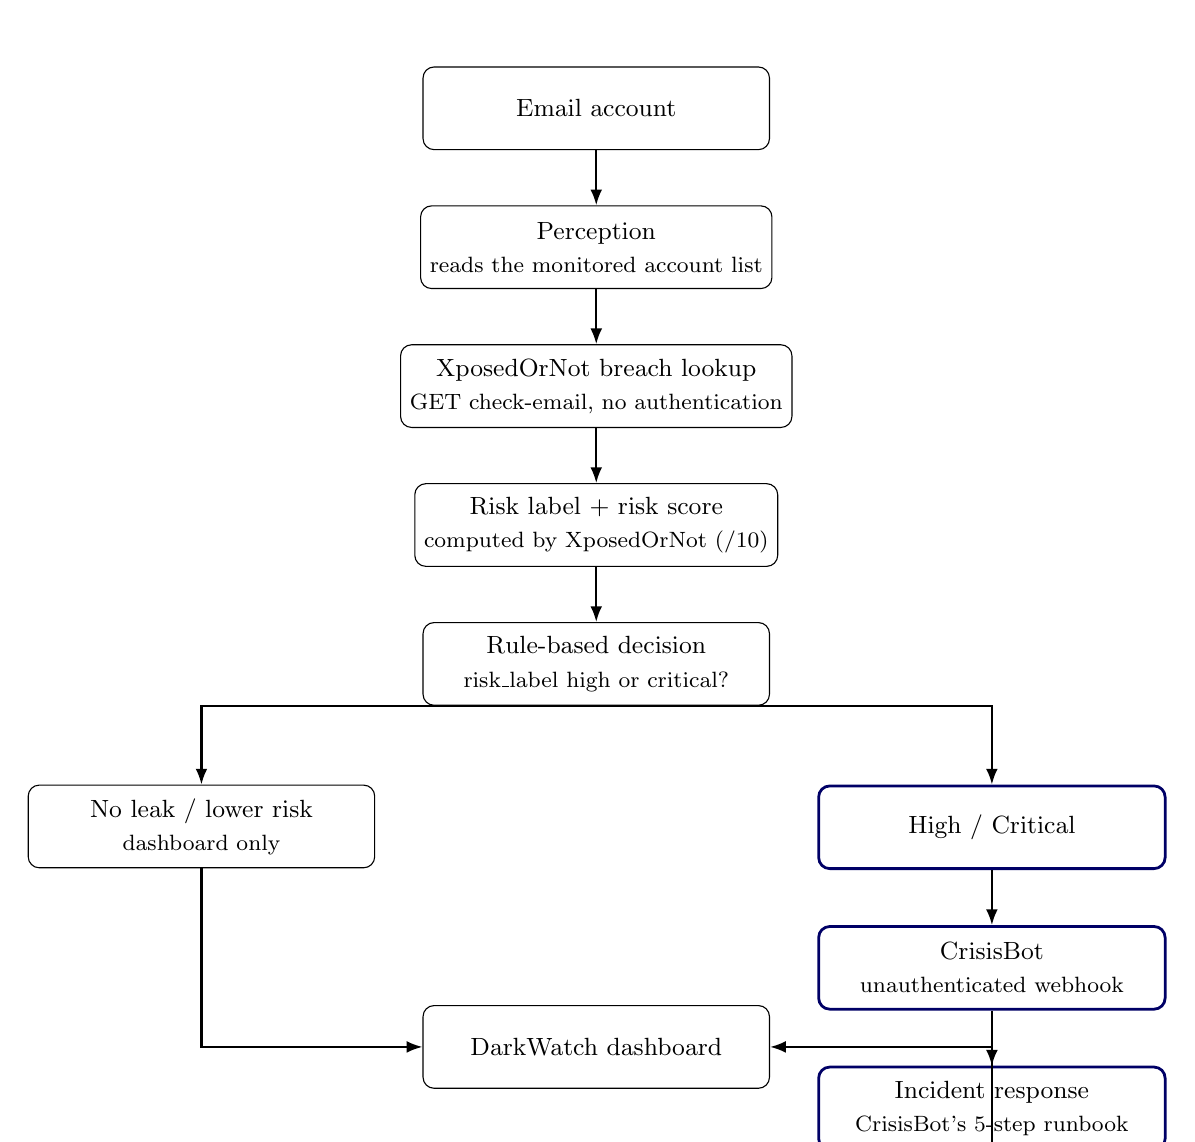
\begin{tikzpicture}[
  box/.style={draw, rounded corners, align=center, minimum width=4.4cm, minimum height=1.05cm, font=\small, fill=white},
  accent/.style={box, draw=blue!40!black, line width=1pt},
  arr/.style={-{Latex[length=2mm]}, thick},
  node distance=7mm and 8mm
]
\node[box] (email) {Email account};
\node[box, below=of email] (perception) {Perception\\[1pt]\footnotesize reads the monitored account list};
\node[box, below=of perception] (lookup) {XposedOrNot breach lookup\\[1pt]\footnotesize GET check-email, no authentication};
\node[box, below=of lookup] (risk) {Risk label + risk score\\[1pt]\footnotesize computed by XposedOrNot (/10)};
\node[box, below=of risk] (decision) {Rule-based decision\\[1pt]\footnotesize risk\_label high or critical?};
\node[box, below left=10mm and 6mm of decision] (noleak) {No leak / lower risk\\[1pt]\footnotesize dashboard only};
\node[accent, below right=10mm and 6mm of decision] (highrisk) {High / Critical};
\node[accent, below=of highrisk] (crisisbot) {CrisisBot\\[1pt]\footnotesize unauthenticated webhook};
\node[accent, below=of crisisbot] (incident) {Incident response\\[1pt]\footnotesize CrisisBot's 5-step runbook};
\node[box, below=38mm of decision] (dash) {DarkWatch dashboard};

\draw[arr] (email) -- (perception);
\draw[arr] (perception) -- (lookup);
\draw[arr] (lookup) -- (risk);
\draw[arr] (risk) -- (decision);
\draw[arr] (decision.south) -| (noleak.north);
\draw[arr] (decision.south) -| (highrisk.north);
\draw[arr] (highrisk) -- (crisisbot);
\draw[arr] (crisisbot) -- (incident);
\draw[arr] (noleak.south) |- (dash.west);
\draw[arr] (incident.south) |- (dash.east);
\end{tikzpicture}
\caption{DarkWatch --- integrated pipeline (\texttt{server.py}, the path actually launched by the project's demo)}
\label{fig:darkwatch-pipeline-main}
\end{figure}

\begin{figure}[htbp]
\centering
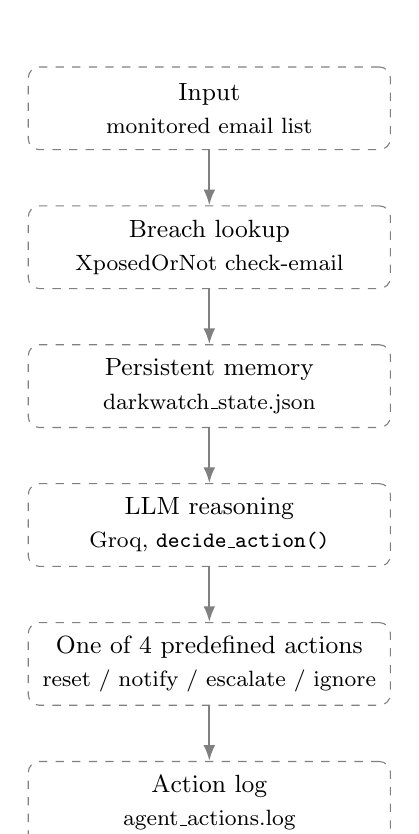
\begin{tikzpicture}[
  box/.style={draw, rounded corners, align=center, minimum width=4.6cm, minimum height=1.05cm, font=\small, fill=white, draw=gray, dashed},
  arr/.style={-{Latex[length=2mm]}, thick, draw=gray},
  node distance=7mm
]
\node[box] (input) {Input\\[1pt]\footnotesize monitored email list};
\node[box, below=of input] (lookup2) {Breach lookup\\[1pt]\footnotesize XposedOrNot check-email};
\node[box, below=of lookup2] (memory) {Persistent memory\\[1pt]\footnotesize darkwatch\_state.json};
\node[box, below=of memory] (reasoning) {LLM reasoning\\[1pt]\footnotesize Groq, \texttt{decide\_action()}};
\node[box, below=of reasoning] (actions) {One of 4 predefined actions\\[1pt]\footnotesize reset / notify / escalate / ignore};
\node[box, below=of actions] (log) {Action log\\[1pt]\footnotesize agent\_actions.log};

\draw[arr] (input) -- (lookup2);
\draw[arr] (lookup2) -- (memory);
\draw[arr] (memory) -- (reasoning);
\draw[arr] (reasoning) -- (actions);
\draw[arr] (actions) -- (log);
\end{tikzpicture}
\caption[DarkWatch --- standalone autonomous mode]{DarkWatch --- standalone autonomous mode (\texttt{agent.py}, a separate script not launched by the project's demo; the \texttt{reset\_password} and \texttt{escalate\_ciso} actions additionally notify CrisisBot)}
\label{fig:darkwatch-pipeline-agent}
\end{figure}

\subsection*{Continuous monitoring and memory}
DarkWatch does not use a learned memory, only a state cache, and the exact mechanism differs by entry point. The command-line script and the standalone agent persist a JSON file (\texttt{darkwatch\_state.json}) across runs so that only newly-seen breaches are reported. The dashboard's background auto-scan loop (enabled only in the project's simulation mode) keeps an in-memory set to avoid repeated notifications within a single session, but this set --- unlike the JSON file --- is lost on restart; manual scans triggered directly from the dashboard keep no memory at all and re-evaluate every account each time.

\subsection*{Integration with CrisisBot}
On a high-risk breach, DarkWatch issues a plain \texttt{POST} to CrisisBot's \code{/api/webhook/incident} endpoint, with a 3-second timeout and no authentication of any kind on either side of the call --- a limitation worth flagging explicitly rather than assuming a project-wide shared-secret convention applies uniformly to every agent. The call is deliberately best-effort: if CrisisBot is unreachable, the exception is caught, a message is printed to the console, and DarkWatch continues operating normally, with no retry.

\subsection*{From data to display}
On the DarkWatch dashboard, each monitored email is listed with a status indicator that starts as ``Waiting...''. When a scan runs, each row updates in place to either ``OK -- no leak found'' or ``Leak detected'', styled in red. If a leak is detected, an alert panel appears below the list, showing: the name(s) of the breach(es), the computed risk label and score, the optional AI-generated summary (clearly labeled as such), and a button to trigger a (simulated, in this demo context) password reset action for that account. A separate search bar also lets a user type any single email address and get an immediate result, using the exact same underlying check.

\subsection*{Limitations}
DarkWatch depends entirely on a single external API; the free-tier quota figures quoted in this section (2 requests/second, 25/hour, 100/day per IP) are those documented in the project's own code and README, not an independently re-verified, currently-live XposedOrNot policy, and should be treated as a project-internal reference rather than an external fact. Coverage is limited to breaches XposedOrNot has already indexed publicly. There is no real Active Directory/Microsoft Graph connection (only a documented, unimplemented code skeleton). Neither the CrisisBot call nor the dashboard itself is authenticated. Storage is local-file-based, with no database. The password-reset action is fully simulated.

\subsection*{Conclusion}
DarkWatch is a non-ML cybersecurity agent whose value comes from automation and integration rather than from a trained model: continuous checking that a human analyst would not realistically repeat by hand, and a direct, if currently unauthenticated, escalation path into CrisisBot's incident-response runbook. Its two levels of automation --- a deterministic, fully auditable integrated mode, and a separate, structurally-constrained autonomous mode where an LLM genuinely selects the final action --- also make it, alongside PhishHunter, one of the two places in \ProjectName{} where a language model is deliberately allowed to decide rather than only explain. The next section turns to NetScope, the first agent in the project that relies on a genuinely trained model.

\section{NetScope --- DNS Anomaly Detection}

\subsection*{Introduction}
NetScope addresses a specific cybersecurity problem: telling an ordinary DNS lookup apart from one that statistically resembles data exfiltration or command-and-control traffic. DNS tunneling encodes data --- credentials, files, stolen records --- into the domain name of a DNS query, then sends it to a server the attacker controls; because DNS traffic is high-volume and rarely inspected in depth, this is hard to catch by hand, and hard to catch with a static blocklist since the domain name itself may never have been seen before. Unlike DarkWatch and CrisisBot, which need no trained model at all, NetScope is a genuinely trained supervised classifier --- one of several agents in \ProjectName{} built around a model learned from labeled data rather than deterministic rules or an external lookup. What makes it architecturally interesting is that it is really two things joined together: an \textbf{offline training process} (a notebook, run on Kaggle against a public labeled dataset, whose only job is to produce a model file) and an \textbf{always-on production service} (\texttt{netscope\_project/}, in this repository) that loads that model and applies it continuously to live-looking traffic. Every technical claim about the production code in this section was verified directly against \texttt{src/netscope\_agent/}; claims that only the notebook can settle are flagged explicitly where the notebook itself is not present in this repository to re-check.

\subsection*{Role in the \ProjectName{} Architecture}
NetScope is an independent web service (FastAPI, its own port) launched alongside the other four agents. Like NetScope's siblings, it does not communicate directly with any other detection agent; its only outbound link is to CrisisBot, triggered automatically once a score clears a fixed bar. Three separate entry points can feed a DNS query into the same pipeline, which mirrors the pattern already seen with DarkWatch's own three entry points:

\begin{itemize}[nosep]
\item \textbf{\texttt{POST /analyze}} --- on-demand scoring, features already supplied by the caller (used by the dashboard).
\item \textbf{\texttt{POST /webhook/traffic-event}} --- a push endpoint for an external firewall or proxy, protected by a shared secret checked with \texttt{hmac.compare\_digest}. If the caller only supplies a domain name, the 16 features are computed live instead of being rejected.
\item \textbf{\texttt{auto\_scan.py}} --- a pull-based autonomous loop that samples a domain roughly every 25 seconds and can act on its own once a score crosses a threshold, the same principle as DarkWatch's \texttt{agent.py}.
\end{itemize}

Whichever entry point fires, the query passes through the same four stages --- perception, feature extraction, scoring, decision --- before reaching one of two outcomes, shown in Figure~\ref{fig:netscope-pipeline}.

\begin{figure}[htbp]
\centering
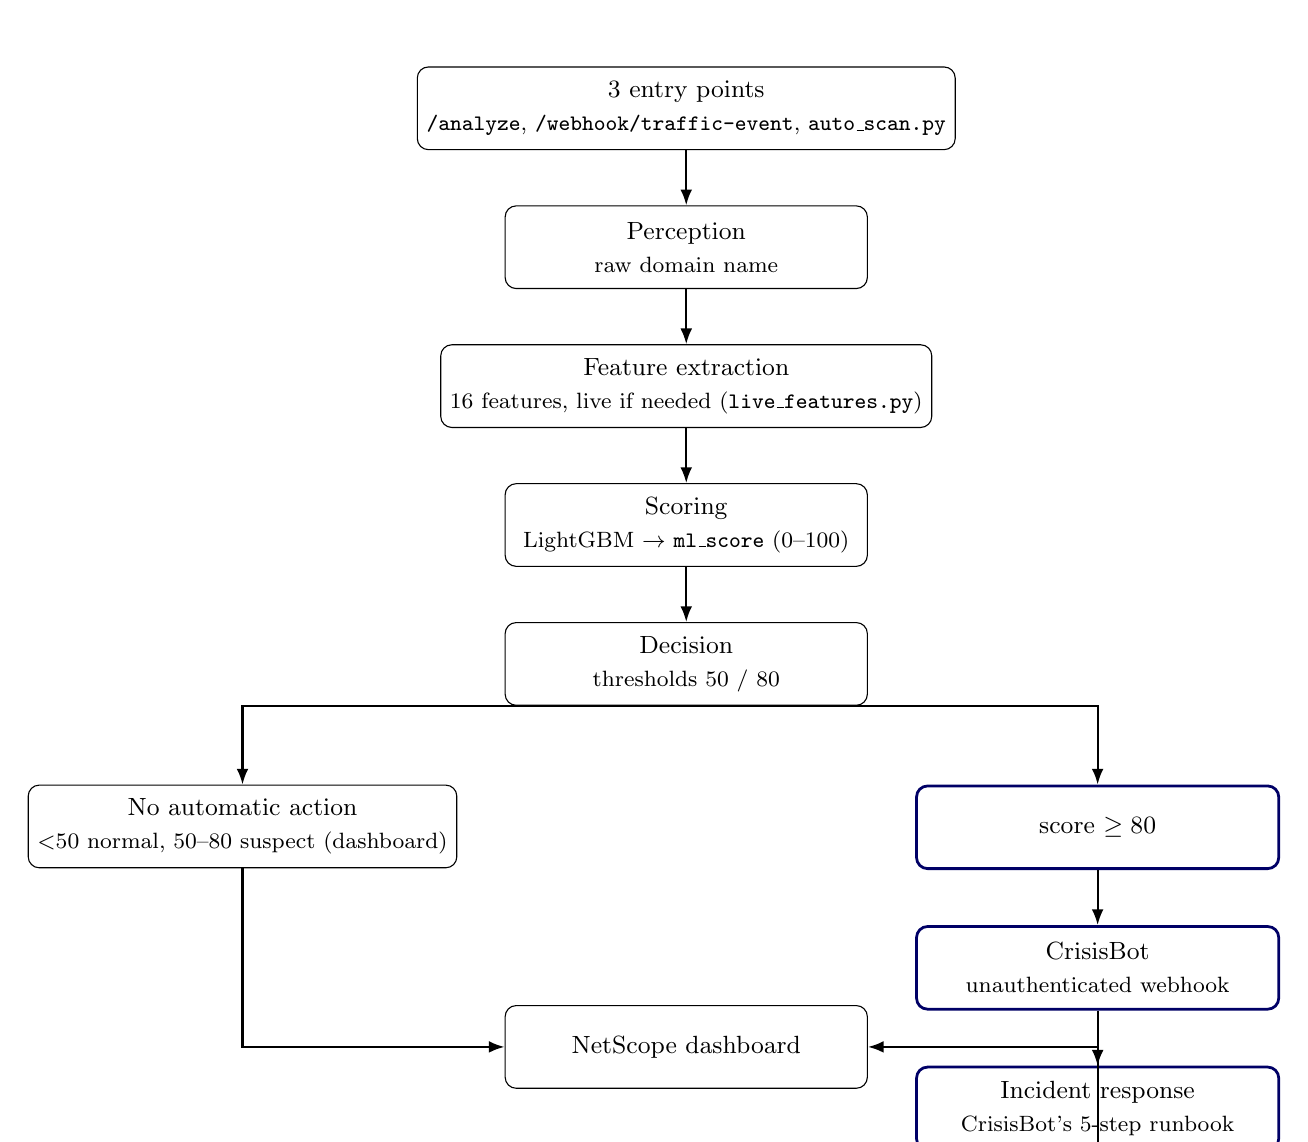
\begin{tikzpicture}[
  box/.style={draw, rounded corners, align=center, minimum width=4.6cm, minimum height=1.05cm, font=\small, fill=white},
  accent/.style={box, draw=blue!40!black, line width=1pt},
  arr/.style={-{Latex[length=2mm]}, thick},
  node distance=7mm and 8mm
]
\node[box] (entries) {3 entry points\\[1pt]\footnotesize \texttt{/analyze}, \texttt{/webhook/traffic-event}, \texttt{auto\_scan.py}};
\node[box, below=of entries] (perception) {Perception\\[1pt]\footnotesize raw domain name};
\node[box, below=of perception] (features) {Feature extraction\\[1pt]\footnotesize 16 features, live if needed (\texttt{live\_features.py})};
\node[box, below=of features] (scoring) {Scoring\\[1pt]\footnotesize LightGBM $\rightarrow$ \texttt{ml\_score} (0--100)};
\node[box, below=of scoring] (decision) {Decision\\[1pt]\footnotesize thresholds 50 / 80};
\node[box, below left=10mm and 6mm of decision] (noaction) {No automatic action\\[1pt]\footnotesize $<$50 normal, 50--80 suspect (dashboard)};
\node[accent, below right=10mm and 6mm of decision] (highscore) {score $\geq 80$};
\node[accent, below=of highscore] (crisisbot) {CrisisBot\\[1pt]\footnotesize unauthenticated webhook};
\node[accent, below=of crisisbot] (incident) {Incident response\\[1pt]\footnotesize CrisisBot's 5-step runbook};
\node[box, below=38mm of decision] (dash) {NetScope dashboard};

\draw[arr] (entries) -- (perception);
\draw[arr] (perception) -- (features);
\draw[arr] (features) -- (scoring);
\draw[arr] (scoring) -- (decision);
\draw[arr] (decision.south) -| (noaction.north);
\draw[arr] (decision.south) -| (highscore.north);
\draw[arr] (highscore) -- (crisisbot);
\draw[arr] (crisisbot) -- (incident);
\draw[arr] (noaction.south) |- (dash.west);
\draw[arr] (incident.south) |- (dash.east);
\end{tikzpicture}
\caption{NetScope --- pipeline (\texttt{src/netscope\_agent/}), styled to mirror DarkWatch's Figure~\ref{fig:darkwatch-pipeline-main}: a single decision point branches into a plain path (dashboard only) and an accented path that reaches CrisisBot automatically once the score clears 80.}
\label{fig:netscope-pipeline}
\end{figure}

Worked example: an external firewall sends \texttt{POST /webhook/traffic-event?x\_webhook\_secret=...} with \texttt{\{"domain": "xj4k9z-relay.info"\}} and no features attached. The shared secret is checked first; since no \texttt{features} dict was supplied, \texttt{extract\_all\_features\_live()} computes all 16 (10 from the domain string alone, 6 from a real DNS resolution). Say the model returns an \texttt{ml\_score} of 87: it clears both the 50 verdict threshold (``suspect'') and the 80 auto-action threshold, so the host is isolated automatically, with no human in the loop for this particular case.

Unlike DarkWatch (no trained model at all) or PhishHunter (an LLM in the decision loop), NetScope is a classic supervised classification pipeline at its core: the model is trained offline, exported, and loaded once at service startup to score requests in real time. The LLM used later in this section never touches the classification decision --- it only writes about a result the model has already produced.

\subsection*{Technical Approach --- Two Halves of One Pipeline}
As in the introduction, NetScope splits cleanly into an offline half and an online half, and the codebase implements this as a genuine handoff rather than a blurred line:

\begin{itemize}[nosep]
\item \textbf{Offline training} (a Kaggle notebook, not stored in this repository): loads the public dataset, selects and justifies 16 features out of 44 raw columns, compares five model families under cross-validation, tunes the winner with Optuna, and exports \texttt{netscope\_model.pkl} and \texttt{netscope\_features.pkl}.
\item \textbf{Online serving} (\texttt{src/netscope\_agent/scorer.py} and the modules around it): loads those two exported files once at startup, reconstructs the same 16 features from nothing but a domain name when a real caller does not supply them, and applies the decision, explanation, and response logic on every query.
\end{itemize}

The rest of this section follows that same order --- dataset, features, model, then the production logic built on top of it --- rather than treating the notebook and the running service as two separate stories.

\subsection*{Dataset and Data Preparation}
The model was trained on the \textbf{CIC-Bell-DNS-Exfiltration 2021} dataset (\texttt{dhoogla/cicbelldnsexf2021} on Kaggle), a public dataset built specifically for DNS exfiltration detection. It ships in six variants --- two cleaning methods (``minimalistic'' and ``opinionated'') crossed with three volumes (``clean-Heavy'', ``clean-BenignExtra'', ``clean-Light''). The training notebook loads the \texttt{minimalistic-clean-Light.parquet} variant; only its two exported artifacts are copied into \texttt{models/} for the production service to load (see \texttt{models/README.md}), so this section reports what the notebook's own cells and markdown commentary state rather than something re-run for this audit.

The raw file holds \textbf{102,762 DNS queries} described by \textbf{44 columns}, including per-record-type frequency statistics (\texttt{A\_frequency}, \texttt{NS\_frequency}, \texttt{CNAME\_frequency}, and others), domain name structure statistics, TTL statistics, and two original label columns: \texttt{GlobalClass} and \texttt{SubClass}. \texttt{GlobalClass} takes the values \texttt{"Light Benign"} and \texttt{"Light Attack"}. The notebook reduces this to a binary \texttt{target} column, with the reasoning spelled out directly in a markdown cell: NetScope needs to answer one simple question --- is this domain suspicious or not --- so \texttt{GlobalClass} is collapsed into two values (0 = Benign, 1 = Attack). Across the 102,762 rows, the real split is \textbf{60,088 Benign} against \textbf{42,674 Attack}, a moderate imbalance (58.5\,\% / 41.5\,\%) rather than an extreme one. This binary \texttt{target} is exactly what \texttt{scorer.py} reproduces in production --- \texttt{model.predict\_proba(x)[0][1]} is the model's estimate of \texttt{target = 1} (Attack) for one query, turned into the 0--100 \texttt{ml\_score} every downstream stage relies on.

Before training, the notebook checks for missing values (\texttt{isnull().sum()}) and duplicate rows (\texttt{duplicated().sum()}). No missing values were found on the label-related columns (\texttt{GlobalClass}, \texttt{SubClass}, \texttt{target}); the exact duplicate-row count the notebook prints could not be independently re-verified in this session, since the notebook itself is not stored in this repository and only runs on Kaggle.

\subsection*{DNS Features}
Of the 44 raw columns, 16 were kept for training. The notebook's own justification: keep the numeric columns that describe a domain name and its DNS query statistically --- name entropy, length, subdomain count, share of digits and special characters, TTL statistics --- rather than the raw domain string itself, which a model like this cannot use directly. These exact same 16 names, in this exact order, are what \texttt{netscope\_features.pkl} exports and what \texttt{NetScopeScorer} demands from every caller in production (\texttt{score\_domain()} raises an explicit error, rather than silently filling a NaN, if any one of the 16 is missing) --- the feature contract is not renegotiated between training and serving.

\begin{table}[h]
\centering
\small
\begin{tabular}{@{}p{3cm}p{4.8cm}p{5.5cm}@{}}
\toprule
\textbf{Feature} & \textbf{What it measures} & \textbf{Why it matters for DNS security} \\
\midrule
\texttt{entropy} & Shannon entropy of the full domain name & A name generated to encode data reads as more random than one a human would choose. \\

\texttt{rr\_name\_entropy} & Entropy of the name inside the DNS resource record & Same signal as \texttt{entropy}, computed one layer closer to the actual DNS packet. \\

\texttt{rr\_name\_length} & Length of the name inside the resource record & Exfiltration techniques encode data into the name, which pushes its length toward the protocol's upper limit. \\

\texttt{len} & Total length of the domain name (FQDN) & Same reasoning: an unusually long name is a classic tunneling signal. \\

\texttt{FQDN\_count} & Number of components in the full domain name & An unusual chain of subdomains can signal encoded data rather than a legitimate naming hierarchy. \\

\texttt{subdomain\_length} & Length of the subdomain portion & Exfiltration typically encodes data in the subdomain rather than the registered domain. \\

\texttt{subdomain} & Whether a subdomain is present (derived indicator) & Reinforces the signal already carried by \texttt{subdomain\_length}. \\

\texttt{labels} & Number of labels (dot-separated segments) in the name & An unusual number of segments is a structural hint of encoding. \\

\texttt{labels\_max} & Length of the longest single label & An abnormally long label rarely occurs in ordinary human naming. \\

\texttt{labels\_average} & Average label length & A complementary signal, less sensitive to a single extreme label than \texttt{labels\_max}. \\

\texttt{numeric} & Share of numeric characters in the name & Base32/base64/hex-encoded data leaves an unusual proportion of digits compared to a normal domain name. \\

\texttt{special} & Share of special characters in the name & Same reasoning as \texttt{numeric}: encoded data leaves a statistical trace in the name's character composition. \\

\texttt{rr\_count} & Number of resource records in the DNS response & An unusual response volume can signal a channel being used to carry more data per query than normal. \\

\texttt{a\_records} & Number of A records in the response & Some exfiltration or C2 techniques abuse A records to carry data or signal status. \\

\texttt{ttl\_mean} & Average TTL of the DNS records observed & Infrastructure tied to malicious activity often uses very short TTLs (fast-flux) or otherwise atypical TTLs compared to legitimate traffic. \\

\texttt{ttl\_variance} & Variance of TTL across observed records & High TTL variance can betray an unstable or deliberately shifting infrastructure, typical of attack infrastructure. \\
\bottomrule
\end{tabular}
\caption{The 16 features NetScope uses to score a DNS query.}
\end{table}

These 16 columns are convenient during training because the dataset already provides them. A real firewall or proxy, in production, only ever hands over a domain name --- it does not pre-compute Shannon entropy or TTL variance. \texttt{live\_features.py} closes this gap, treating the 16 features as two families: \textbf{10 name-only features} (\texttt{entropy}, \texttt{len}, \texttt{FQDN\_count}, \texttt{subdomain\_length}, \texttt{subdomain}, \texttt{numeric}, \texttt{special}, \texttt{labels}, \texttt{labels\_max}, \texttt{labels\_average}), computable from the domain string alone, and \textbf{6 DNS-response features} (\texttt{rr\_name\_entropy}, \texttt{rr\_name\_length}, \texttt{rr\_count}, \texttt{a\_records}, \texttt{ttl\_mean}, \texttt{ttl\_variance}), which require an actual DNS resolution against a public resolver and fall back to 0 --- rather than raising --- if \texttt{dnspython} is missing or the resolution fails. The module's own documentation is explicit about the one feature it cannot faithfully reconstruct: \texttt{ttl\_variance} is always 0 on this live path, because a single DNS resolution only ever yields a single TTL value --- a true variance would need several observations spread over time, which this synchronous request/response flow does not have.

This live-resolution path is also what the project's real-phone demonstration is built on: a local DNS proxy (\texttt{dns\_proxy.py}) transparently relays a phone's DNS traffic while logging each queried domain, and a log-tailing bridge (\texttt{tail\_bridge.py}) pushes each new domain to \texttt{/webhook/traffic-event} in near real time, so the dashboard's live-feed panel reflects genuine phone browsing rather than a canned sample --- see \emph{From Data to Display} below.

\subsection*{Feature Engineering and Selection}
The notebook does not simply fix the 16 features up front and move on. It ranks them by importance (using the \texttt{feature\_importances\_} of a trained Random Forest), then re-runs the comparison keeping only the top 8 to see how much performance is lost.

\begin{table}[h]
\centering
\small
\begin{tabular}{@{}lc@{}}
\toprule
\textbf{Feature} & \textbf{Importance (Random Forest)} \\
\midrule
\texttt{FQDN\_count}        & 0.174 \\
\texttt{subdomain\_length}  & 0.133 \\
\texttt{special}            & 0.126 \\
\texttt{numeric}            & 0.124 \\
\texttt{ttl\_mean}          & 0.121 \\
\texttt{labels}             & 0.115 \\
\texttt{labels\_average}    & 0.042 \\
\texttt{labels\_max}        & 0.029 \\
\texttt{rr\_count}          & 0.029 \\
\texttt{rr\_name\_entropy}  & 0.026 \\
\texttt{ttl\_variance}      & 0.025 \\
\texttt{rr\_name\_length}   & 0.022 \\
\texttt{subdomain}          & 0.015 \\
\texttt{len}                & 0.010 \\
\texttt{entropy}            & 0.009 \\
\texttt{a\_records}         & 0.000 \\
\bottomrule
\end{tabular}
\caption{Feature importance from the Random Forest trained in the notebook.}
\end{table}

Dropping to the top 8 features barely moves the result: F1 = 0.8309 with all 16 features against F1 = 0.8301 with only 8. Six features (\texttt{FQDN\_count}, \texttt{subdomain\_length}, \texttt{special}, \texttt{numeric}, \texttt{ttl\_mean}, \texttt{labels}) already carry more than 79\,\% of the total importance. The model that actually gets exported --- and the one \texttt{scorer.py} loads in production --- keeps all 16 features rather than this reduced set, which is why \texttt{live\_features.py} still has to reconstruct all 16 and not just the top 8.

\subsection*{Machine Learning Model}
Several model families were tested and compared. A first, simple pass (Random Forest and XGBoost on a single train/test split) gives close results (accuracy 0.835 for both). Before going further, the notebook checks whether a trained model is even worth the trouble, by testing a naive rule: flag a domain as suspicious if its entropy exceeds 3.5. That rule reaches an accuracy of 0.582 but an F1 of only 0.0236 (precision 0.388, recall 0.012) --- it misses almost every real attack. On the same test set, the trained models clear 0.83 F1, which is the honest answer to whether the model --- and the entire production pipeline built around it --- earns its complexity.

The notebook then compares five models with 5-fold stratified cross-validation on F1 and ROC-AUC:

\begin{table}[h]
\centering
\small
\begin{tabular}{@{}lcccc@{}}
\toprule
\textbf{Model} & \textbf{F1 mean} & \textbf{F1 (std)} & \textbf{ROC-AUC mean} & \textbf{ROC-AUC (std)} \\
\midrule
LightGBM              & 0.8312 & 0.0017 & 0.8704 & 0.0012 \\
XGBoost                & 0.8309 & 0.0016 & 0.8707 & 0.0012 \\
Random Forest           & 0.8309 & 0.0017 & 0.8698 & 0.0011 \\
HistGradientBoosting    & 0.8308 & 0.0017 & 0.8707 & 0.0009 \\
Logistic Regression     & 0.8221 & 0.0015 & 0.8685 & 0.0021 \\
\bottomrule
\end{tabular}
\caption{Five-fold stratified cross-validation across five supervised models.}
\end{table}

Worth stating plainly: the four tree/boosting models are practically indistinguishable --- the gap between the best and the worst of the four is under 0.05 F1 points, smaller than their own standard deviation. Only logistic regression, the simplest model, clearly trails behind. Picking LightGBM owes more to a marginal edge and training/inference speed than to any real performance gap over the other tree-based models. This choice also has a direct production consequence: \texttt{NetScopeScorer} builds a \texttt{shap.TreeExplainer}, which works cleanly for LightGBM (and the other tree/boosting models tested) but would fail for logistic regression --- one more reason the tree-based family, not just LightGBM specifically, was the right lane to stay in.

LightGBM's hyperparameters were then tuned with \textbf{Optuna} (Bayesian search, 50 trials) rather than an exhaustive grid --- a \texttt{GridSearchCV} had already been used earlier in the notebook, but only for a preliminary Random Forest tuning pass, and the notebook itself notes that grid search is ``expensive and coarse'' compared to a Bayesian search for the final tuning step. Optuna's best hyperparameters: \texttt{n\_estimators=112}, \texttt{max\_depth=6}, \texttt{learning\_rate$\approx$0.144}, \texttt{num\_leaves=51}, \texttt{min\_child\_samples=23}, \texttt{subsample$\approx$0.946}, \texttt{colsample\_bytree$\approx$0.547}, \texttt{reg\_alpha$\approx$1.01}, \texttt{reg\_lambda$\approx$9.65e-8}, with a cross-validated F1 of \textbf{0.8313}. The tuned model beat the base LightGBM in the comparison, so it is the one exported (the notebook prints: ``Best model: tuned LightGBM (CV F1 = 0.8313)''). On the held-out test set, its classification report reads:

\begin{table}[h]
\centering
\small
\begin{tabular}{@{}lcccc@{}}
\toprule
\textbf{Class} & \textbf{Precision} & \textbf{Recall} & \textbf{F1} & \textbf{Support} \\
\midrule
0 (Benign) & 1.00 & 0.72 & 0.84 & 12,018 \\
1 (Attack) & 0.72 & 1.00 & 0.83 & 8,535 \\
\midrule
Accuracy & \multicolumn{4}{c}{0.84} \\
\bottomrule
\end{tabular}
\caption{Classification report of the final tuned LightGBM model on the test set.}
\end{table}

Read honestly, this table means the model misses zero attacks on this test set (recall = 1.00 on the Attack class) at the cost of a real false-positive rate (precision = 0.72, so roughly 28\,\% of benign traffic gets flagged). In a security context, trading precision for recall this way is generally the right call --- missing a real exfiltration attempt is more costly than chasing a false alarm, though this reading is not stated as a deliberate design goal anywhere in the notebook itself and should be treated as an observation made after the fact, not a documented objective. It also foreshadows a production choice: with a model this willing to flag benign traffic, the service cannot afford to act automatically on every ``suspect'' verdict --- exactly why the production code, not the notebook, introduces a second, much higher bar before anything happens without a human (see Risk Scoring and Decision, below).

The final model and its 16-feature list are exported with \texttt{joblib} (\texttt{netscope\_model.pkl}, \texttt{netscope\_features.pkl}). This is the handoff point between the two halves of NetScope: everything before this line happened once, offline, on Kaggle; everything after it happens continuously, in \texttt{src/netscope\_agent/}, every time a query is scored.

\subsection*{Risk Scoring and Decision}
\texttt{NetScopeScorer.\_\_init\_\_} loads both exported files once at service startup (\texttt{joblib.load}) and raises a clear \texttt{FileNotFoundError} pointing to \texttt{models/README.md} if they are missing, rather than failing obscurely later. \texttt{score\_domain()} then does exactly what the notebook's final classification report measured: \texttt{proba = model.predict\_proba(x)[0][1]}, turned into \texttt{ml\_score = round(proba * 100, 1)} --- the single number every other stage of the pipeline (thresholds, SHAP, the LLM, the dashboard) is built around.

The production code, not the notebook, is where the actual decision logic lives, and it uses \textbf{two separate thresholds} that should not be confused with each other:

\begin{itemize}[nosep]
\item \textbf{50.0} --- the verdict threshold (\texttt{NetScopeScorer.threshold} in \texttt{scorer.py}): above it, a query is labeled \texttt{"suspect"} instead of \texttt{"normal"} for display purposes.
\item \textbf{80.0} --- \texttt{AUTO\_ACT\_THRESHOLD} in \texttt{auto\_scan.py}: above it, the system isolates the host and notifies CrisisBot \emph{automatically}, without waiting for a human to click anything. This same threshold and constant gate both the autonomous pull loop and the push webhook (\texttt{api.py} imports \texttt{AUTO\_ACT\_THRESHOLD} directly from \texttt{auto\_scan.py} rather than redefining it).
\end{itemize}

A third, purely cosmetic level exists only for the dashboard: \texttt{risk\_level()} buckets the score into four labels (Low $<$30, Medium $<$60, High $<$80, Critical $\geq$80), with no effect on any decision.

The three-term composite score explored in the training notebook (0.7 × ML score + 0.2 × traffic score + 0.1 × human score) \textbf{does not exist in the production code}. The score used everywhere in the running service is simply \texttt{ml\_score = round(proba × 100, 1)}. A user's simulated human risk profile --- looked up deterministically from a fictional directory, \texttt{data/users.json}, via a SHA-256 hash of the hostname (\texttt{get\_user\_for\_host} in \texttt{actions.py}), standing in for a real HR or phishing-simulation platform such as GoPhish or KnowBe4 --- shapes the wording of the recommendation shown to the analyst (through \texttt{human\_priority()}, which buckets the profile's own risk score into ``élevée'' $\geq$70, ``moyenne'' $\geq$40, or ``faible'' below that), not a blended numeric score.

\subsection*{SHAP Explainability}
This is a case where the notebook and the production code disagree, and the production code is the one that matters here. SHAP never appears in the training notebook --- but the running service genuinely uses it. \texttt{NetScopeScorer} builds a \texttt{shap.TreeExplainer(self.model)} at startup, and every scored query goes through an \texttt{explain()} call that returns the top 4 features driving that particular decision, each tagged with a direction (increases or decreases risk). These get translated into analyst-readable labels via a fixed dictionary in \texttt{scorer.py} (\texttt{"rr\_name\_entropy"} $\rightarrow$ \emph{``Entropie du nom de domaine élevée''}) and shown on the dashboard as ``Main factors''. The code degrades gracefully (\texttt{self.explainer = None}, and \texttt{explain()} then returns an empty list instead of raising) if \texttt{TreeExplainer} fails to build --- relevant for a model like logistic regression, tested in the model comparison above but not the one ultimately kept, which is precisely why that comparison mattered for more than just picking the highest F1.

\subsection*{Role of the LLM}
NetScope also calls an LLM (Groq, \texttt{llama-3.1-8b-instant}), but strictly for writing, never for deciding --- the system prompt forbids it explicitly: ``Ne jamais reclasser l'alerte (suspect/normal) : c'est déjà décidé en amont'' (\emph{never reclassify the alert: that decision has already been made upstream}). The LLM receives the score already computed, the SHAP factors already computed, and the human risk profile already looked up, and produces only a natural-language explanation and a recommended action, returned as strict JSON with exactly two keys (\texttt{explanation}, \texttt{recommendation}). With no Groq API key configured, or if the call fails or returns something outside that shape, a template-based fallback (\texttt{\_template\_fallback} in \texttt{llm.py}) builds the same kind of explanation from the same real data --- the same SHAP factors, the same score, the same human-priority bucket --- never inventing anything. This role --- explain, never decide --- lines up with the principle already stated in Chapter~2, and puts NetScope alongside DarkWatch's integrated mode and PhishHunter's deterministic path as places where a language model narrates a decision it never made.

\subsection*{Continuous Monitoring and Memory}
NetScope does not use a learned memory either, only a lightweight in-process cache, and like DarkWatch the exact mechanism differs by entry point. \texttt{auto\_scan.py} keeps an in-memory set, \texttt{\_already\_acted}, of domains already isolated automatically during the current run, so the same domain is not re-isolated on every subsequent draw of the sample; the push webhook (\texttt{/webhook/traffic-event}) checks and updates the same module-level set, so a domain isolated via one entry point is not re-isolated via the other. This set --- exactly like DarkWatch's in-memory deduplication set for its background auto-scan loop --- is lost on restart: nothing here is persisted to disk, so a fresh process re-evaluates every domain as if seeing it for the first time. On-demand scoring through \texttt{/analyze} keeps no memory at all and never triggers automatic isolation regardless of score, by design --- that endpoint only ever returns a score for the dashboard to display.

\subsection*{Integration with CrisisBot}
A single shared function, \texttt{actions.record\_isolation}, logs the incident (\texttt{data/incidents.json}, with \texttt{domain}, \texttt{user}, \texttt{ml\_score}, a timestamp, and a \texttt{source} tag) and notifies CrisisBot, regardless of whether it was triggered by a human click (\texttt{POST /isolate}), the autonomous loop, or the push webhook --- so the incident only gets logged once no matter which of the three entry points fired it. The notification itself (\texttt{crisisbot\_client.py}) follows the same best-effort pattern seen with DarkWatch and the other detection agents: a plain \texttt{POST} to \texttt{CRISISBOT\_URL} (\texttt{/api/webhook/incident}), a 3-second timeout, and \textbf{no authentication of any kind on either side of the call} --- the exception is caught, a message is printed to the console, and NetScope continues operating normally, with no retry, exactly the same limitation already flagged for DarkWatch rather than a NetScope-specific gap.

\subsection*{From Data to Display}
The NetScope dashboard (\texttt{static/index.html}) opens with a dark ``traffic card'' labeled as coming from a firewall/proxy webhook (Fortinet, PaloAlto are named as examples), listing domains fetched from \texttt{GET /sample-traffic?n=4} with their \texttt{ml\_score} shown as a percentage; rows flagged \texttt{"suspect"} are highlighted in red with a warning icon. Every domain shown here is resolved live through a real DNS lookup rather than sampled from a static file, and the feed always includes at least one currently active, publicly reported malicious domain (drawn from the URLhaus/abuse.ch public threat-intelligence feed) mixed in with legitimate and synthetically generated domains, so the demonstration is not limited to fabricated examples. A second panel, ``Trafic en direct'' (live traffic), polls \texttt{GET /live-feed} every two seconds and displays events pushed through \texttt{/webhook/traffic-event} in near real time --- including, when the local DNS proxy/tail-bridge demonstration described above is running, genuine DNS queries made by a real phone. Each row in this panel is clickable and opens the same detailed score view described below.

The page always focuses on the first suspect result in that sample: its domain, its NetScope risk score and colored level badge (Faible/Moyen/Élevé/Critique), and its SHAP ``main factors'' list, each prefixed with a \texttt{+} or \texttt{--} sign for the direction it pushed the score. Below that, a profile card shows the correlated user's name, department, and human risk score, followed by a one-sentence correlation message whose wording depends on that user's priority bucket (élevée / moyenne / faible) --- the same three-way bucket produced by \texttt{human\_priority()} described above under Risk Scoring and Decision. A single ``Isoler le poste'' button calls \texttt{POST /isolate} and, on success, confirms the exact timestamp and states explicitly that the incident was logged to \texttt{data/incidents.json} --- the same shared function described above, this time with \texttt{source="manual"}.

\subsection*{Limitations}
All five supervised models compared share the same structural limit: they only recognize attacks that statistically resemble what is already present in CIC-Bell-DNSExF2021. A genuinely new DNS exfiltration technique, never represented in that dataset, could slip through undetected --- a limit of the offline training data that no amount of production engineering around it can change. \texttt{live\_features.py} documents an honest limitation of its own on the production side: \texttt{ttl\_variance} is always 0 on the live path, since a single DNS resolution only yields a single TTL, and its reconstruction of the DNS response features is a reasonable approximation, not a certified match to the original dataset authors' exact methodology --- a gap between the offline features the model learned from and the online features it is actually served in production, even though both are computed from the same 16 definitions. Neither the CrisisBot call nor the dashboard itself is authenticated, the same limitation already noted for DarkWatch. The project's own \texttt{README.md} still lists verifying the absence of data leakage in the features among its next steps --- something this audit did not re-verify and that remains an open question. The live phone demonstration (\texttt{dns\_proxy.py}/\texttt{tail\_bridge.py}) is also a local, single-machine setup built for a live defense demo, not a production-grade network tap --- it relays raw DNS bytes and never modifies them, but was not designed or hardened for deployment on a real corporate network.

\subsection*{Conclusion}
NetScope pairs a conventional but carefully built machine learning pipeline --- five model families compared under cross-validation, Bayesian hyperparameter tuning, and an explicit sanity check against a naive rule --- with a production layer that closes the gap between a research dataset and a real domain name (\texttt{live\_features.py}), adds real SHAP explainability, and lets an LLM write but never decide. The two thresholds that actually drive behavior, 50 for the suspect/normal verdict and 80 for automatic isolation, live entirely in the service code, not the training notebook, and neither matches a single ``80/100'' figure loosely used elsewhere. As a supervised classifier, NetScope remains bound by what its training data has already seen, a limitation the project's own code and documentation acknowledge rather than hide. The next section turns to PhishHunter, the only other agent in \ProjectName{} built around a trained model, and the one where --- unlike NetScope's LLM, confined to writing --- a language model is deliberately allowed a second, genuinely agentic decision path of its own.

\section{PhishHunter --- Phishing Email Detection Agent}

\subsection*{Non-technical idea}
PhishHunter reads an incoming email the way a suspicious human would: it looks both at \emph{what the email says} (urgent language, threats about account suspension, generic greetings) and at \emph{where it really comes from} (a domain that looks almost, but not quite, like a legitimate one). Combining both signals catches more phishing attempts than looking at either alone.

\subsection*{Technical approach --- supervised machine learning (Logistic Regression + text embedding), plus one explicit LLM-based exception}
PhishHunter's scoring engine combines two kinds of input for a single Logistic Regression classifier:

\begin{itemize}[nosep]
\item \textbf{12 handcrafted tabular features}, confirmed in \texttt{src/features/extract.py}: presence of urgency language (\texttt{has\_urgency}), number of URLs in the body (\texttt{url\_count}), presence of an IP-address-based URL rather than a domain name (\texttt{has\_ip\_url}), word count (\texttt{word\_count}), similarity of the sender's domain to a known brand via Levenshtein distance (\texttt{is\_typosquat}, \texttt{typosquat\_distance}), domain-name entropy (\texttt{domain\_entropy}), domain length (\texttt{domain\_length}), ratio of digits in the domain (\texttt{domain\_digit\_ratio}), ratio of uppercase characters in the body (\texttt{uppercase\_ratio}), count of exclamation marks (\texttt{exclamation\_count}), and whether sender information is present at all (\texttt{has\_sender\_info}).
\item \textbf{A 200-dimensional Word2Vec embedding} of the email text, mean-pooled into a single vector, which lets the model capture semantic patterns in the wording itself rather than only surface-level statistics.
\end{itemize}

Both feature groups are concatenated into a single input vector fed to the classifier, which outputs the final \texttt{risk\_score} (0--100); a human-readable explanation is separately generated by an LLM based on which signals were triggered --- again, the LLM only \emph{writes}, it does not decide the score.

PhishHunter is the one explicit, deliberate exception, in this project, to the principle that ``the LLM never decides alone'': it includes an optional \emph{autonomous agent mode}. In this mode, a large language model (Llama 3.3 70B, accessed through the Groq API) is given the already-computed score and triggered signals, and must choose, through structured \emph{tool calling}, exactly one of three predefined final actions: \texttt{block\_email}, \texttt{escalate\_to\_human}, or \texttt{deliver\_normally}. Structured tool calling means the model can only select from a fixed, predefined list of functions --- it cannot invent a new action, and the actual Python code behind each function is what really executes, not the model's text output. If the case is ambiguous, the agent may first call an auxiliary \texttt{check\_domain\_age} tool (a live WHOIS lookup) before deciding. As a safety net, if the LLM call itself fails for any reason (a known intermittent issue with structured function calling), the system automatically falls back to \texttt{escalate\_to\_human} rather than leaving the email unprocessed or silently failing.

The project's own \texttt{README.md} states that the final model was trained on a corpus of \textbf{163,700 emails drawn from 7 combined sources}. The exact composition of those 7 sources, and the training notebook itself (run on Kaggle, per the same convention as NetScope and Sentinel), could not be located with certainty among the files accessible during this internship, so \TODO{the precise per-source breakdown and the original notebook, if retrievable}.

\begin{figure}[htbp]
\centering
\includesvg[inkscapelatex=false,width=0.95\textwidth]{phishhunter_pipeline}
\caption{PhishHunter agent pipeline}
\label{fig:phishhunter-pipeline}
\end{figure}

\subsection*{From data to display}
\begin{flushleft}
The PhishHunter dashboard lists received emails with a colored score badge (green/amber/red depending on the score range) next to the sender and subject. Selecting an email opens a detail panel with the full score, classification, and the natural-language explanation of why it was flagged. A ``Block email and alert employee'' button lets an analyst act directly on the score-based recommendation, while a separate ``Let the agent decide'' button triggers the autonomous mode described above: the dashboard then displays the agent's reasoning trace step by step, showing each tool it called (with its input and result formatted in plain readable lines rather than raw JSON, and long WHOIS text automatically truncated for readability), ending with the final decision clearly highlighted (e.g. ``Decision: block the email'').
\end{flushleft}

% =====================================================
\section{Sentinel --- Insider Threat Detection Agent}

\subsection*{Non-technical idea}
Sentinel is not looking for an external attacker; it is looking for behavior from a legitimate account that does not match that account's usual pattern --- logging in at 3 a.m. from a device never seen before, for example. This is the classic insider-threat problem: the credentials are valid, so the anomaly has to be detected from \emph{context} (time, device, department) rather than from a password being wrong.

\subsection*{Technical approach --- unsupervised machine learning (Isolation Forest)}
Sentinel uses a fundamentally different kind of machine learning than NetScope or PhishHunter: it is \textbf{unsupervised}, meaning the model was never given labelled examples of ``this is an insider threat'' during training --- because in real insider-threat data, such clean labels almost never exist. The model used is an Isolation Forest, trained on the \textbf{CERT Insider Threat Dataset} (Carnegie Mellon University, roughly 3.5 million raw logged events).

The intuition behind Isolation Forest, in plain terms: the algorithm repeatedly splits the data with random cuts, and it measures, for each point, how many random cuts it takes to isolate that point completely on its own. A ``normal'' login resembles many other logins in the dataset, so it takes many cuts to separate it from the crowd. An unusual login (e.g. an unheard-of hour combined with a brand-new device) resembles almost nothing else, so it gets isolated in very few cuts --- and the fewer cuts needed, the higher the anomaly score.

The raw CERT dataset was deliberately reduced from many raw fields down to \textbf{7 ``universal'' features}, confirmed in the production code (\texttt{feature\_engineering.py}): a cyclical encoding of the hour of day (\texttt{hour\_sin}, \texttt{hour\_cos}, via sine/cosine transforms so that, e.g., 23:00 and 00:30 are recognized as close together rather than as opposite extremes), a weekend flag (\texttt{is\_weekend}), a public-holiday flag (\texttt{is\_holiday}), an off-hours flag (\texttt{is\_off\_hours}), a sensitive-department flag (\texttt{is\_sensitive\_department}), and a new-device flag (\texttt{is\_new\_device}). The CERT dataset is publicly documented as originally containing raw records of user, workstation, and logon/logoff events; in this project, this raw data was reduced during preprocessing to the seven features listed above.

This reduction is an intentional design choice: by keeping only features that exist in essentially any identity system (Entra ID, Google Workspace, etc.), the trained model was shown, in the notebook, to transfer to a different, fabricated identity-provider sample without any retraining --- a property that would not hold if the model depended on CERT-specific fields. A Tunisia-specific recalibration was also applied to the definition of ``business hours'' used by the \texttt{is\_off\_hours} feature.

Sentinel's decision engine then applies \textbf{differentiated thresholds} depending on whether the account belongs to a sensitive department (e.g. Finance, Compliance, IT Management, General Management): for a normal account, scores below 25 trigger no action, 25--55 puts the account under monitoring, 55--85 automatically assigns targeted security training, and above 85 escalates to a human analyst (which also notifies CrisisBot). For a sensitive-department account, the same four thresholds are lowered to 15/40/65, so an identical anomaly is treated more strictly when it involves a higher-privilege account.

On the concurrency side, the production service is built to keep serving scoring requests reliably even while a background retraining job is running or many requests arrive at once: the currently active model is held behind an immutable, atomically-swapped state object, so a request in flight is never affected mid-read by a model being replaced; writes (a retrain completing) are serialized behind a non-blocking lock, so a second retrain signal arriving while one is already running is coalesced rather than starting a competing job; and retraining itself runs on a single persistent background worker thread, gated so it only fires once enough new cases have accumulated (rather than retraining on every single request), instead of spawning a new thread per request.

\begin{figure}[htbp]
\centering
\includesvg[inkscapelatex=false,width=0.95\textwidth]{sentinel_pipeline}
\caption{Sentinel agent pipeline}
\label{fig:sentinel-pipeline}
\end{figure}

\subsection*{From data to display}
Sentinel's dashboard presents a set of selectable login ``cases'' as chips; selecting one populates a dark, console-style activity feed showing the raw login details. Clicking ``Analyze with Sentinel'' animates the decision pipeline step by step (feature extraction, model scoring, threshold decision), then reveals a result card color-coded by outcome (red for escalation, amber for training, green/neutral for no action), showing the user's name, department, computed risk score, and the plain-language reason for the decision, optionally rewritten by an LLM for readability. A separate ``simulate a live connection'' form lets a user manually enter a custom username, workstation, department, date, and hour, and get an on-the-spot analysis using the exact same model and thresholds. Beyond this manual simulation, Sentinel can also be exercised with genuinely real login events: the six \ProjectName{} dashboards share a single email/password authentication layer, and every successful login across any of them is logged (source agent, timestamp) and can feed Sentinel's analysis pipeline as a real, rather than simulated, connection event.

% =====================================================
\section{CrisisBot --- Automated Incident Response Orchestration}

\subsection*{Non-technical idea}
Once a threat has been detected by any of the four agents above, someone still has to actually \emph{do something about it}: isolate the affected machine, tell the right people, and prepare a message so the rest of the organization is informed without panic. CrisisBot is the agent that carries out this coordinated response automatically and consistently, every time, regardless of which of the four detection agents raised the alarm. It is not a conversational \emph{chatbot}: it is an incident-response orchestrator.

\subsection*{Technical approach --- no machine learning, orchestration and LLM-assisted communication only}
CrisisBot uses \textbf{no machine learning model of any kind}, and this is stated plainly rather than implied: its job is not to detect or classify anything, but to execute a fixed, deterministic five-step \emph{runbook} (confirmed in \texttt{server.py}) whenever it receives an incident notification, summarized in Table~\ref{tab:runbook}.

\begin{table}[htbp]
\centering
\begin{tabular}{@{}>{\raggedright\arraybackslash}p{0.6cm}>{\raggedright\arraybackslash}p{4.2cm}>{\raggedright\arraybackslash}p{7.5cm}@{}}
\toprule
\textbf{\#} & \textbf{Step} & \textbf{Detail} \\
\midrule
1 & Isolate the affected host & Automatic network disconnection of the affected workstation to stop the spread \\
2 & Notify the CISO & Immediate alert sent with the detected indicators of compromise \\
3 & Notify Management & Executive summary sent to allow the crisis cell to be triggered if needed \\
4 & Activate the crisis cell & Automatic convening of IT, security, and communications referents \\
5 & Prepare internal communication & Message ready to inform teams without creating panic \\
\bottomrule
\end{tabular}
\caption{CrisisBot's fixed, five-step runbook}
\label{tab:runbook}
\end{table}

These five steps, and their order, never change --- what changes is only \emph{which} incident triggered them and \emph{who} (which of the four other agents) triggered them.

CrisisBot exposes a webhook endpoint (\texttt{/api/webhook/incident}) that the four detection agents call automatically and directly, with no human in the loop, whenever their own threshold is crossed; a second endpoint (\texttt{/api/simulate}) also lets an analyst trigger the exact same runbook manually from the dashboard, for demonstration or drills. For the final ``prepare communication'' step only, a large language model (via Groq, module \texttt{llm\_comms.py}) may be used to draft the actual wording of the internal announcement, tailored to the specific incident description --- but only the wording is generated by the LLM; whether that step happens at all, and in what order, is entirely fixed by the code, independent of the model. If the LLM is not configured, a generic fallback message is used (\texttt{FALLBACK\_MESSAGE}), and CrisisBot continues to function normally.

\begin{sloppypar}
CrisisBot is also connected to a genuine Slack incoming webhook (module \code{notifications.py}): when properly configured through \code{SLACK_WEBHOOK_URL}, the alert is not merely simulated on screen but is really posted to a live Slack channel, which was verified end-to-end during this internship. The Teams and Email channels shown in the interface remain, at this stage, simulated: \TODO{no real Teams or Email integration was connected during this internship}.
\end{sloppypar}

\subsection*{From data to display}
The CrisisBot dashboard displays the fixed five-step runbook as a checklist; when an incident is processed, each step animates from pending to ``in progress'' to a completed, checked state, with a realistic elapsed-time simulation. A status banner indicates whether the real Slack integration is currently configured or only running in simulated mode. A small set of preset incident types (ransomware, DNS exfiltration, phishing, anomalous connection) can be triggered with one click for demonstration purposes, and a free-text field allows a fully custom incident description. Once the runbook completes, a summary line confirms the total handling time, lists which channels were notified, and explicitly states whether the Slack message was genuinely sent or only simulated --- so the difference between a real and a simulated action is never hidden from the person using the dashboard.

% =====================================================
\section{Interconnections Between Agents and External Integrations}

Table~\ref{tab:integrations} distinguishes, for each external integration considered in this project, what has \textbf{actually been implemented and verified} during this internship from what remains \textbf{conceptualized} (code ready, but never connected to a real production system).

\begin{table}[htbp]
\centering
\footnotesize
\begin{tabularx}{\textwidth}{@{}>{\raggedright\arraybackslash}p{3.4cm}>{\raggedright\arraybackslash}p{2.8cm}>{\raggedright\arraybackslash}X@{}}
\toprule
\textbf{Integration} & \textbf{Status} & \textbf{Detail} \\
\midrule
XposedOrNot (DarkWatch) & Implemented & Real, live API calls, verified during the internship \\
Slack incoming webhook (CrisisBot) & Implemented & Messages genuinely sent to a Slack channel, verified end-to-end \\
Groq API (LLM, several agents) & Implemented & Real calls for drafting summaries/explanations and for PhishHunter's agent mode \\
Public DNS resolution (NetScope) & Implemented & Real DNS resolution via \texttt{dnspython} for live feature computation, plus a local DNS proxy/tail-bridge demonstration relaying a real phone's DNS traffic \\
URLhaus threat-intelligence feed (NetScope) & Implemented & Public list of currently active malicious domains (abuse.ch), merged into the live traffic sample so at least one entry is a real, currently reported threat \\
WHOIS (\code{check_domain_age}, PhishHunter) & Implemented & Real WHOIS lookup used by the autonomous agent mode \\
Generic firewall webhook (NetScope) & Implemented (endpoint), not connected & Endpoint ready to receive events from a real firewall (Fortinet, Palo Alto), but no real firewall has been connected; the local DNS proxy demonstration substitutes for this during the internship \\
Shared login/logout authentication (all 6 dashboards) & Implemented & Email/password session shared across the 6 dashboards via a signed cookie; every login is logged and can feed Sentinel with real (not simulated) connection events \\
Microsoft Graph API (PhishHunter) & Conceptualized & Webhook subscription validation handshake code written and ready, but no real OAuth subscription to a Microsoft 365 mailbox has been established \\
Active Directory / Entra ID (Sentinel) & Conceptualized & No real connection; only the model's reusability on a fabricated Entra ID sample was demonstrated in the notebook \\
SIEM & Conceptualized & No real SIEM connected; documented as an integration prospect \\
Teams / Email notifications (CrisisBot) & Conceptualized & Shown in the interface but simulated, no real integration connected \\
\bottomrule
\end{tabularx}
\caption{External integrations: implemented vs. conceptualized}
\label{tab:integrations}
\end{table}

Table~\ref{tab:datasets} summarizes the datasets used to train the models in this project.

\begin{table}[htbp]
\centering
\begin{tabular}{@{}>{\raggedright\arraybackslash}p{2.6cm}>{\raggedright\arraybackslash}p{3.6cm}>{\raggedright\arraybackslash}p{3.5cm}>{\raggedright\arraybackslash}p{3cm}@{}}
\toprule
\textbf{Agent} & \textbf{Dataset} & \textbf{Size} & \textbf{Origin} \\
\midrule
NetScope & CIC-BellDNS-Exfiltration2021 & 102,762 labelled DNS queries & Canadian Institute for Cybersecurity \\
Sentinel & CERT Insider Threat Dataset & $\sim$3.5 million raw events, reduced to 7 features & Carnegie Mellon University (CERT Division) \\
PhishHunter & Corpus documented in the project's own \texttt{README.md} & 163,700 emails, 7 combined sources & \TODO{exact per-source composition and original Kaggle notebook not located with certainty} \\
DarkWatch & None (no ML, live API call) & --- & --- \\
CrisisBot & None (no ML) & --- & --- \\
\bottomrule
\end{tabular}
\caption{Datasets used to train the project's models}
\label{tab:datasets}
\end{table}

No dataset of Tunisian origin was publicly available for these use cases at the time of the internship: the public datasets above (Canadian for NetScope, American for Sentinel) were therefore used as a training basis, with context-specific adjustments applied afterward (e.g. the business-hours recalibration for Sentinel).

Table~\ref{tab:tech} lists the main technologies used throughout the project.

\begin{table}[htbp]
\centering
\begin{tabular}{@{}>{\raggedright\arraybackslash}p{4cm}>{\raggedright\arraybackslash}p{8.5cm}@{}}
\toprule
\textbf{Category} & \textbf{Technologies} \\
\midrule
Language & Python \\
Web servers & FastAPI (NetScope, PhishHunter, Sentinel); standard-library \texttt{http.server} (DarkWatch, CrisisBot) \\
Machine learning & scikit-learn, LightGBM, XGBoost (comparison), gensim (Word2Vec) \\
Explainability & SHAP \\
LLM & Groq API (Llama 3.3 70B) \\
Network/DNS & dnspython \\
Frontend & HTML/CSS/JavaScript (independent dashboard per agent) \\
\bottomrule
\end{tabular}
\caption{Main technologies used}
\label{tab:tech}
\end{table}

% =====================================================
\section{Evaluation and Results}

This section gathers the performance elements actually confirmed in the project's files (notebooks, code), clearly distinguishing what is quantified from what remains to be completed --- in line with the strict rule of never inventing a metric.

\subsection*{NetScope}
Table~\ref{tab:netscope-cv} reproduces the model comparison carried out through 5-fold stratified cross-validation, already detailed in full under \emph{Machine Learning Model} above. LightGBM's mean cross-validated F1-score (\textbf{0.8312}) and ROC-AUC (\textbf{0.8704}) are the two headline figures for the selected model; the other four models' values are reproduced here for direct side-by-side comparison rather than repeated as a separate, only-partially-confirmed table.

\begin{table}[htbp]
\centering
\begin{tabular}{@{}>{\raggedright\arraybackslash}p{4.5cm}>{\raggedright\arraybackslash}p{4cm}>{\raggedright\arraybackslash}p{4cm}@{}}
\toprule
\textbf{Model} & \textbf{Mean F1 (5-fold CV)} & \textbf{Mean ROC-AUC} \\
\midrule
Logistic Regression & 0.8221 & 0.8685 \\
Random Forest & 0.8309 & 0.8698 \\
HistGradientBoosting & 0.8308 & 0.8707 \\
XGBoost & 0.8309 & 0.8707 \\
\textbf{LightGBM (selected, tuned)} & \textbf{0.8313} & \textbf{0.8704} \\
\bottomrule
\end{tabular}
\caption{NetScope model comparison by cross-validation (all values as reported in the training notebook; the tuned LightGBM figure of 0.8313 is the post-Optuna result, marginally above its own pre-tuning 0.8312)}
\label{tab:netscope-cv}
\end{table}

The notebook also notes that all five supervised models converge toward an F1-score close to 0.83, and that a Bayesian hyperparameter search (Optuna, 50 trials) applied to LightGBM only produced a marginal gain --- suggesting, according to the notebook's own notes, that the performance ceiling comes more from the available data/features than from the model choice or fine-tuning.

\subsection*{Sentinel}
Because Isolation Forest is an unsupervised model, there are no ground-truth labels directly comparable to classic supervised classification metrics (precision/recall) on the training data itself. The qualitative validation carried out in the notebook focused on the trained model's ability to transfer, without retraining, to a fabricated sample representing a different identity provider (Entra ID): this portability test was successful, confirming that the 7 selected features are not specific to the original CERT dataset. \TODO{precise quantitative metrics (ROC-AUC score on a labelled subset, detection rate) could not be confirmed in the accessible files}.

\subsection*{PhishHunter}
\TODO{the precise evaluation metrics (precision, recall, F1, confusion matrix) of PhishHunter's Logistic Regression model could not be confirmed, as the corresponding training notebook could not be located with certainty during this internship}. Real examples observed during testing carried out during the internship (via the simulator) show behavior consistent with the model's objective: clearly fraudulent emails (typosquatted domains such as \texttt{micros0ft-verify.com} or \texttt{paypa1-security.com}) received scores close to 100/100, while legitimate emails received scores close to 0. These are qualitative observations from manual testing, not a formal statistical evaluation on a test set.

\subsection*{DarkWatch and CrisisBot}
\begin{sloppypar}
Since neither of these two agents integrates any machine learning model, no precision/recall-type metric applies: their validation was carried out functionally (the XposedOrNot API responds correctly for an email known to be exposed; CrisisBot's runbook executes in the correct order and the Slack message is actually received on the configured channel), which was verified manually during the internship.
\end{sloppypar}

% =====================================================
\section{Difficulties Encountered and Solutions Applied}

This section honestly describes the main technical difficulties actually encountered while implementing this project, along with the solutions applied.

\begin{itemize}[nosep]
\item \textbf{Race condition in the event simulator}: the demonstration simulator would sometimes mark an agent as ``unreachable'' (status 0) even though it had just started and had not yet finished opening its port. \emph{Solution:} the delay before the first request was increased, and standard-output buffering was disabled for the launched processes, in order to obtain a reliable diagnosis of each agent's actual state.
\item \textbf{Shared-secret comparison vulnerable to timing attacks}: a plain string comparison (\texttt{==}) between the received secret and the expected secret can, in theory, leak information through response time. \emph{Solution:} replaced with \texttt{hmac.compare\_digest}, a constant-time comparison, applied to the NetScope and Sentinel webhooks.
\item \textbf{Malformed JSON request body on CrisisBot's webhook}: an external call sending an invalid or empty JSON body caused an unhandled server-side exception. \emph{Solution:} defensive reading of the request body (\texttt{\_read\_json\_body}) that returns an explicit HTTP 400 response instead of leaving the request unanswered.
\item \textbf{Persistence of the Slack environment variable}: the \texttt{SLACK\_WEBHOOK\_URL} variable, set in a terminal session, did not automatically persist across restarts of the CrisisBot server. \emph{Solution:} explicit documentation of the command to re-run before each startup, and a clear ``configured / not configured'' status shown on the dashboard for the Slack integration, rather than silently hiding the difference between a real and a simulated send.
\item \textbf{Port conflicts when launching all five agents simultaneously}: since each agent starts on a fixed port, two instances launched by mistake on the same machine would conflict. \emph{Solution:} each port is configurable via a dedicated environment variable (e.g. \texttt{CRISISBOT\_PORT}), with an explicit error message suggesting the port-change command when a conflict is detected.
\item \textbf{Intermittent failures of structured function calling (LLM) in PhishHunter}: the \emph{tool calling} call to the Groq API occasionally failed (a \code{tool_use_failed}-type error). \emph{Solution:} automatic fallback to the \code{escalate_to_human} decision on failure, ensuring an email is never left without a decision, even if the LLM is unavailable.
\item \textbf{Shared session cookie broken by the admin email's own format}: after switching the shared login system from a plain username to an email address, authentication silently stopped working across all six dashboards. \emph{Root cause}: the session cookie packed three fields (email, expiry, signature) separated by the character \texttt{.}, and was parsed with a plain \texttt{split(".")} expecting exactly three parts --- but the admin email itself contains a \texttt{.}, producing four parts instead of three and causing every session to be silently rejected. \emph{Solution:} the cookie is now parsed with \texttt{rsplit(".", 2)}, which always isolates the two trailing, delimiter-free fields (expiry, signature) from the right and treats everything remaining on the left as the email, regardless of how many dots it itself contains.
\end{itemize}

Although modest individually, these difficulties illustrate a broader issue representative of multi-agent systems in production: robustness does not come solely from the quality of the machine learning models, but equally from defensive handling of edge cases (networking, concurrency, configuration, external dependencies).

% =====================================================
\section{Current Limitations and Prospects for Future Development}

\subsection*{Current limitations}
\begin{itemize}[nosep]
\item The events processed by the agents during this internship were generated by a controlled simulator rather than by live production systems, since access to real banking infrastructure (mailboxes, identity providers, firewalls) was not available within the scope of the internship. NetScope is a partial exception: its live DNS resolution and its local proxy/tail-bridge demonstration process genuine DNS traffic (including from a real phone), though still outside a real corporate network.
\item No real, active connection was established with Microsoft Exchange/Graph, Active Directory/Entra ID, a production firewall, or a SIEM: these integrations remain at the stage of ready code (see Table~\ref{tab:integrations}), not real deployment.
\item Authentication between agents relies solely on a shared secret compared in constant time: there is no more robust authentication mechanism (mutual certificates, short-lived tokens, automatic secret rotation).
\item The dashboards now sit behind a shared, optional email/password login (a signed cookie, no server-side session store, one demo account, no real user directory): this is a genuine access-control layer, but not a production-grade identity system (no per-user accounts, no password hashing rotation policy, no role-based access control).
\item Data storage (logs, state) relies on local JSON/log files, with no persistent database or automated backup.
\item There is no automatic model retraining pipeline (MLOps), nor continuous integration/deployment (CI/CD).
\item Some precise performance metrics (see Section~2.8) still need to be formally documented using dedicated test sets.
\end{itemize}

\subsection*{Prospects for future development}
\begin{itemize}[nosep]
\item Finalize the real connection to Microsoft Graph (OAuth subscription to a Microsoft 365 mailbox) so that PhishHunter processes real emails rather than simulated ones.
\item Connect Sentinel to a real identity provider (Entra ID) or to a SIEM, building on the already-demonstrated portability of the 7-feature universal model, and continue feeding it with real login events captured through the shared authentication layer.
\item Connect NetScope to a real firewall or proxy (Fortinet, Palo Alto) via the already-ready, vendor-agnostic webhook endpoint, extending the local DNS proxy demonstration toward a production-scale network tap.
\item Activate CrisisBot's Teams and Email notification channels, currently simulated, alongside the already-functional Slack webhook.
\item Implement a more robust inter-agent authentication mechanism than the current static shared secret, and a production-grade identity system (per-user accounts, role-based access) for the dashboards themselves.
\item Add a persistent database and a backup mechanism, replacing the current JSON/log file storage.
\item Formally document each model's performance metrics on dedicated test sets, and implement model-drift monitoring over time.
\end{itemize}

\section*{Conclusion}
Taken together, these five activities allowed me to design and implement a coherent multi-agent security system, applying a consistent architectural pattern while adapting the specific technique --- supervised learning, unsupervised learning, external API lookups, or pure orchestration --- to the nature of each threat, and being explicit, in every case, about which parts genuinely use machine learning and which do not. It is worth noting honestly that, during this internship, the events processed by the agents were generated by a controlled simulator rather than by live production systems; the detection, scoring, decision, and notification logic itself is fully functional and was designed from the start to accept real events through the same webhook interfaces, without requiring any redesign.

% =====================================================
% GENERAL CONCLUSION
% =====================================================

\chapter*{General Conclusion}
\addcontentsline{toc}{chapter}{General Conclusion}
\markboth{General Conclusion}{}

This internship at Hydatis gave me the opportunity to work on a complete, realistic cybersecurity project, combining several disciplines that are usually studied separately: supervised and unsupervised machine learning, natural language processing through large language models, API integration, and system architecture design.

Beyond the technical skills acquired --- building and evaluating ML models, integrating real external services, designing webhook-based architectures, and using LLMs responsibly within an automated decision pipeline --- this experience also strengthened my ability to explain complex technical systems clearly, to be honest about the limitations of a given implementation, and to plan concretely how a prototype could evolve toward a production-ready system.

\TODO{personal closing paragraph to enrich with your own reflections on this internship}

I leave this internship with a much clearer understanding of how modern, AI-driven cybersecurity systems are designed in practice, and with strong motivation to continue developing my skills in this field.

% =====================================================
% BIBLIOGRAPHY / WEBOGRAPHY
% =====================================================

\chapter*{Bibliography and Webography}
\addcontentsline{toc}{chapter}{Bibliography and Webography}

\begin{itemize}[nosep]
\item XposedOrNot --- public data-breach lookup API. \url{https://xposedornot.com}
\item Canadian Institute for Cybersecurity --- CIC-BellDNS-Exfiltration2021 dataset. \url{https://www.unb.ca/cic/datasets/}
\item Carnegie Mellon University, CERT Division --- CERT Insider Threat Dataset. \url{https://www.cert.org}
\item Groq --- LLM inference API documentation. \url{https://console.groq.com/docs}
\item scikit-learn --- official documentation. \url{https://scikit-learn.org}
\item LightGBM --- official documentation. \url{https://lightgbm.readthedocs.io}
\item SHAP (SHapley Additive exPlanations) --- official documentation. \url{https://shap.readthedocs.io}
\item gensim --- Word2Vec documentation. \url{https://radimrehurek.com/gensim/}
\item Microsoft Graph API --- official documentation (integration considered, not finalized). \url{https://learn.microsoft.com/graph}
\item Slack --- incoming webhooks documentation. \url{https://api.slack.com/messaging/webhooks}
\item URLhaus (abuse.ch) --- public malware-URL/domain threat-intelligence feed used by NetScope's live-feed demonstration. \url{https://urlhaus.abuse.ch}
\item dnspython --- DNS toolkit documentation, used for NetScope's live DNS resolution and the local DNS proxy demonstration. \url{https://www.dnspython.org}
\end{itemize}

\TODO{complete this list with any other source actually consulted during the internship}

% =====================================================
% APPENDICES
% =====================================================
\appendix
\chapter*{Appendices}
\addcontentsline{toc}{chapter}{Appendices}
\markboth{Appendices}{}

\section*{Appendix A --- Example webhook call to CrisisBot}
\begingroup\small
\begin{verbatim}
POST /api/webhook/incident
Content-Type: application/json

{
  "source_agent": "netscope",
  "severity": "high",
  "description": "Suspected DNS exfiltration toward a high-entropy domain"
}
\end{verbatim}
\endgroup

\section*{Appendix B --- Example of features sent to NetScope ("pre-computed features" mode)}
\begingroup\small
\begin{verbatim}
{
  "entropy": 3.91, "len": 42, "FQDN_count": 4,
  "subdomain_length": 18, "subdomain": 1, "numeric": 6,
  "special": 0, "labels": 4, "labels_max": 18,
  "labels_average": 9.5, "rr_name_entropy": 3.7,
  "rr_name_length": 42, "rr_count": 1, "a_records": 1,
  "ttl_mean": 300, "ttl_variance": 0
}
\end{verbatim}
\endgroup

\section*{Appendix C --- List of PhishHunter's 12 tabular features (exact model order)}
\begingroup\small
\begin{verbatim}
has_urgency, url_count, has_ip_url, word_count, is_typosquat,
typosquat_distance, domain_entropy, domain_length, domain_digit_ratio,
uppercase_ratio, exclamation_count, has_sender_info
\end{verbatim}
\endgroup

\end{document}
